%!TEX root = informe.tex
\chapter{Análisis de Ciclo de Vida de un adoquín: interpretación}\label{cap:acv_interpretacion}

Es la fase del ACV en la que los resultados del ICV y el EICV son interpretados de acuerdo al objetivo y alcance marcados inicialmente. En esta fase se realiza un análisis de los resultados y se marcan las conclusiones.

\section{Verificación del análisis de integridad}

El objetivo de esta verificación es ``asegurar que stoda la información y datos pertinentes necesarios para la interpretación están disponibles y completos'' \cite{iso14044}. La integridad asegura que no se ha olvidado ningún aspecto importante conocido.

Se ha verificado que todos los procesos unitarios de todas las fases, comprobando entradas y salidas, energía, transporte y residuos.

\section{Verificación del análisis de sensibilidad}

Hasta ahora, para calcular el perfil ambiental se ha utilizado el método ReCiPe desde la perspectiva jerárquica H. Para realizar un análisis de sensibilidad se compararán por fases los resultados con las otras perspectivas mencionadas en la sección \ref{sec:catimpactos}, la individualista (I) y la igualitaria (E).

La figura \ref{fig:sensibilidad_ia_puntuacionunica} y la tabla \ref{sensibilidad_ia_puntuacionunica} muestran los resultados usando la perspectiva individualista (I).

\begin{figure}[!htb]
\centering
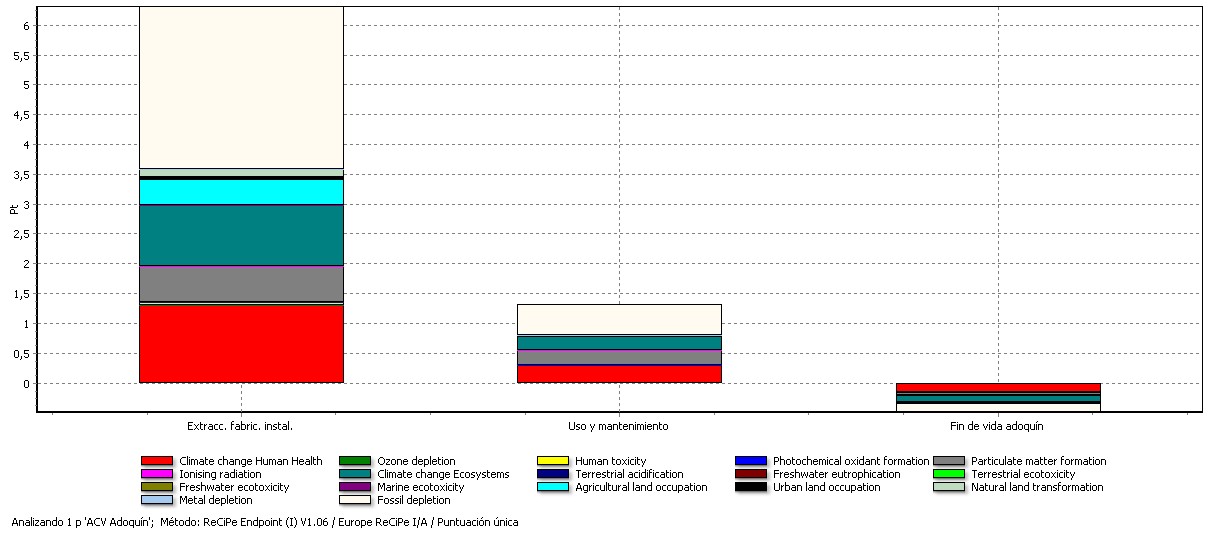
\includegraphics[width=15cm]{img/sensibilidad_ia_puntuacionunica.png}
\caption{Puntuación única por categorías de daño con el método ReCiPe I/A.}
\label{fig:sensibilidad_ia_puntuacionunica}
\end{figure}

\begin{table}[!htb]
\centering
\begin{tabular}{p{6cm}rrrr}
\toprule
\multicolumn{5}{c}{Categorías de daño ReCiPe I/A}\\
\midrule
Etapa & Salud hum. & Ecosistema & Recursos & Total\\
 & (Pt) & (Pt) & (Pt) & (Pt)\\
\midrule
Extracc., fabric. e instal. & 7900 & 4010 & 6720 & 18600\\
Uso y mantenim. & 0.55 & 0.25 & 0.52 & 1.32\\
Fin de vida & -6.69 & -4.09 & -7.47 & -18.30\\
\bottomrule
\end{tabular}
\caption{Puntuación única por categorías de daño con el método ReCiPe I/A.}
\label{sensibilidad_ia_puntuacionunica}
\end{table}
La figura \ref{fig:sensibilidad_ia_puntuacionunica} y la tabla \ref{sensibilidad_ia_puntuacionunica} muestran los resultados usando la perspectiva individualista (I).

Por otro lado, la figura \ref{fig:sensibilidad_ea_puntuacionunica} y la tabla \ref{sensibilidad_ea_puntuacionunica} muestran los resultados usando la perspectiva igualitaria (E).

\begin{figure}[!htb]
\centering
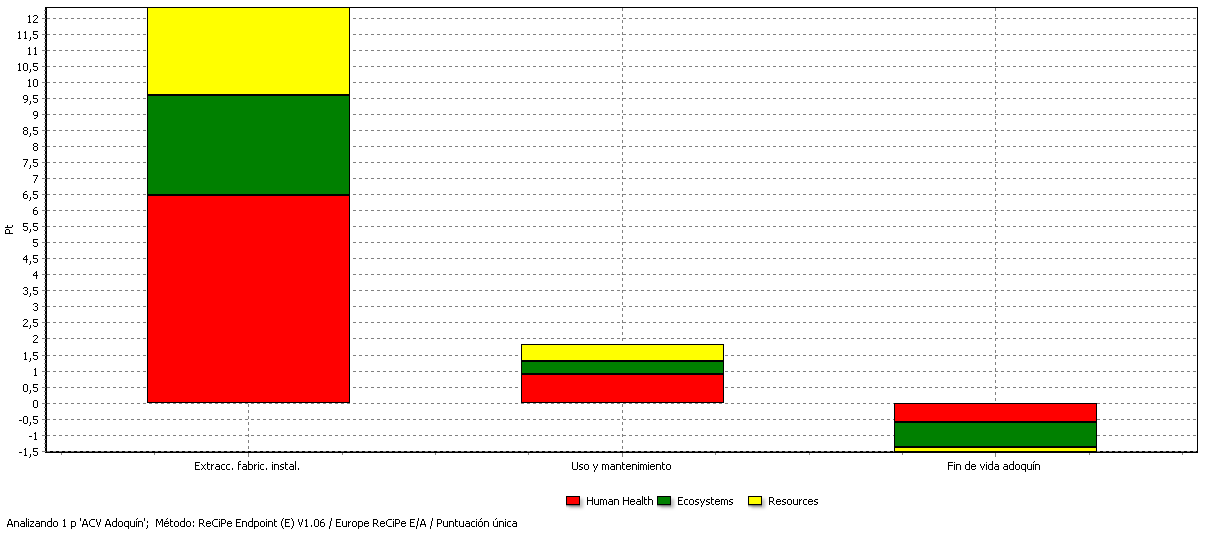
\includegraphics[width=15cm]{img/sensibilidad_ea_puntuacionunica.png}
\caption{Puntuación única por categorías de daño con el método ReCiPe E/A.}
\label{fig:sensibilidad_ea_puntuacionunica}
\end{figure}

\begin{table}[!htb]
\centering
\begin{tabular}{p{6cm}rrrr}
\toprule
\multicolumn{5}{c}{Categorías de daño ReCiPe E/A}\\
\midrule
Etapa & Salud hum. & Ecosistema & Recursos & Total\\
 & (Pt) & (Pt) & (Pt) & (Pt)\\
\midrule
Extracc., fabric. e instal. & 44600 & 8690 & 6540 & 59800\\
Uso y mantenim. & 0.88 & 0.44 & 0.52 & 1.84\\
Fin de vida & -14 & -7.73 & -8.57 & -30.30\\
\bottomrule
\end{tabular}
\caption{Puntuación única por categorías de daño con el método ReCiPe E/A.}
\label{sensibilidad_ea_puntuacionunica}
\end{table}

La comparación de los resultados entre las tres perspectivas de la tabla \ref{comparativa_perspectivas} indica que las perspectivas jerárquicas e individualista tienen resultados similares, mientras que la igualitaria se diferencia bastante. Mientras que la perspectiva individualista es a corto plazo y optimista en cuanto a que la tecnología puede evitar muchos problemas en el futuro, la perspectiva igualitaria se basa a largo plazo y en una forma de pensar precavida, considerando a la naturaleza frágil e inestable, una visión fatalista poco aceptada, por lo que podría ser descartada para este proyecto, y aceptar esta parte del análisis de sensibilidad como superado.

\begin{table}[!htb]
\centering
\begin{tabular}{p{6cm}rrr}
\toprule
\multicolumn{4}{c}{Comparativa de perspectivas}\\
\midrule
Etapa & I/A & H/A & E/A\\
 & (Pt) & (Pt) & (Pt)\\
\midrule
Extracc., fabric. e instal. & 18600 & 20900 & 59800\\
Uso y mantenim. & 1.32 & 1.4 & 1.84\\
Fin de vida & -18.30 & -18.40 & -30.30\\
\bottomrule
\end{tabular}
\caption{Comparativa de perspectivas H, I, E a nivel del puntuación única por categorías de daño con el método ReCiPe.}
\label{comparativa_perspectivas}
\end{table}

El análisis de sensibilidad necesita además un análisis de incertidumbre utilizando el método ReCiPe H/A con el ``Análisis Monte Carlo''. El análisis Monte Carlo es una manera numérica de procesar datos inciertos y de establecer un rango de incertidumbre en el resultado del cálculo.

\begin{figure}[!htb]
\centering
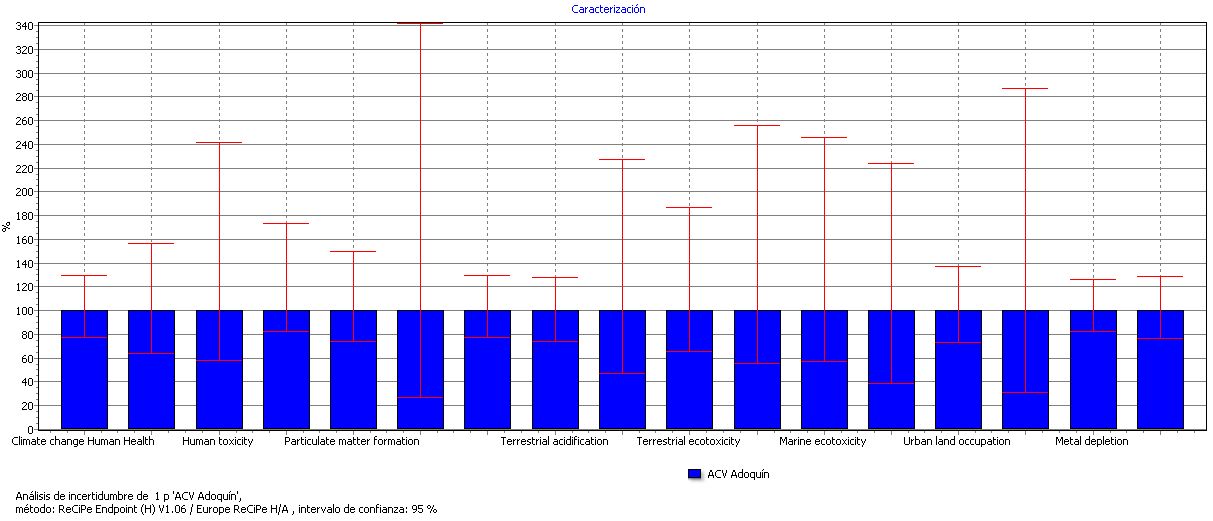
\includegraphics[width=15cm]{img/confianza_caracterizacion.png}
\caption{Intervalos de confianza para cada categoría de impacto a nivel de caracterización del ACV del adoquín.}
\label{fig:confianza_caracterizacion}
\end{figure}

Por cada categoría de impacto se indica un diagrama de barras con un margen de incertidumbre. El margen manifiesta el 95\% del intervalo de confiabilidad, lo que significa que el 95\% de los resultados estuvo dentro de este margen. Las figuras \ref{fig:confianza_caracterizacion},\ref{fig:confianza_normalizacion},\ref{fig:confianza_puntuacionunica} y \ref{fig:confianza_dano} muestran que los resultados del Análisis de Ciclo de Vida tienen una confianza del 95\%.

\begin{figure}[!htb]
\centering
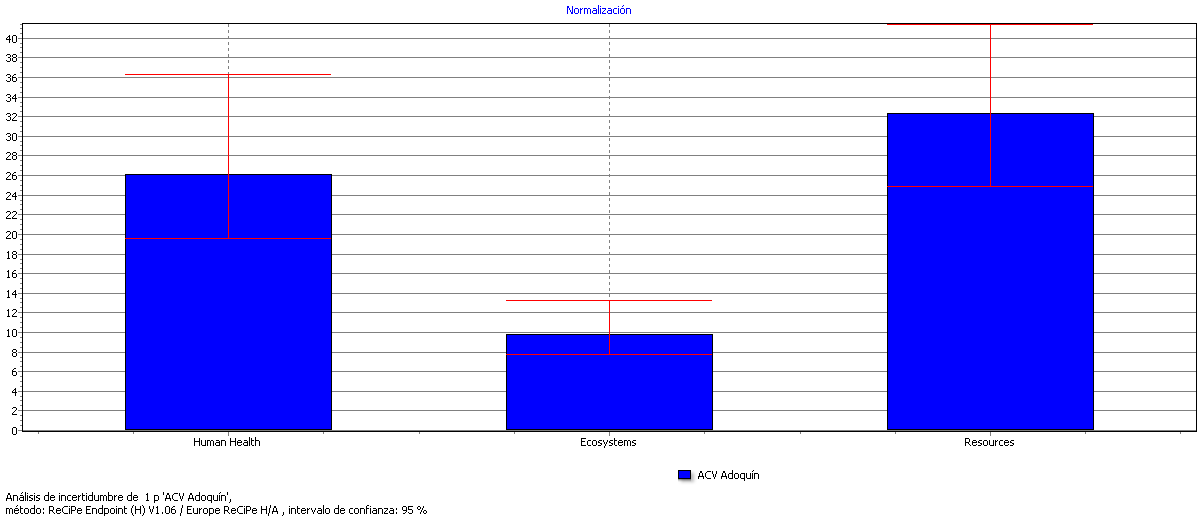
\includegraphics[width=15cm]{img/confianza_normalizacion.png}
\caption{Intervalos de confianza para cada categoría de impacto normalizada del ACV del adoquín.}
\label{fig:confianza_normalizacion}
\end{figure}

\begin{figure}[!htb]
\centering
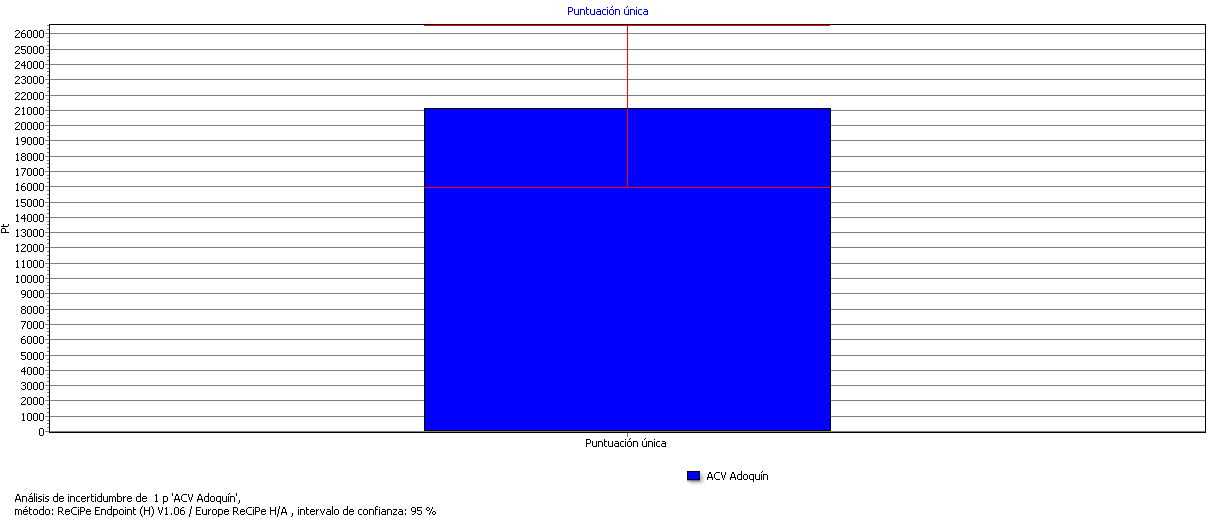
\includegraphics[width=15cm]{img/confianza_puntuacionunica.png}
\caption{Intervalos de confianza para cada categoría de impacto a nivel de puntuación única del ACV del adoquín.}
\label{fig:confianza_puntuacionunica}
\end{figure}

\begin{figure}[!htb]
\centering
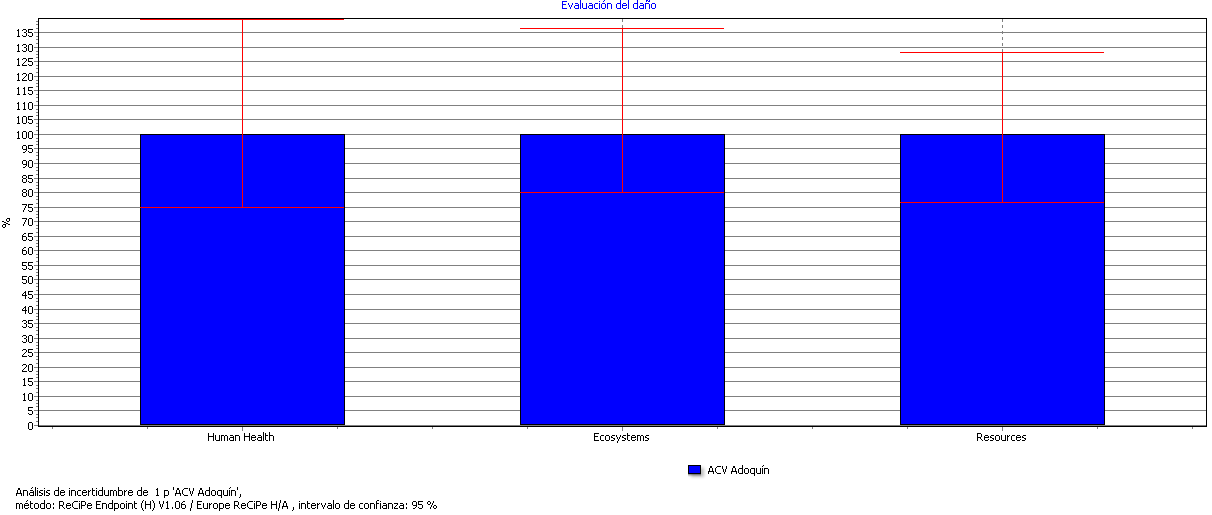
\includegraphics[width=15cm]{img/confianza_dano.png}
\caption{Intervalos de confianza para cada categoría de daño a nivel de puntuación única del ACV del adoquín.}
\label{fig:confianza_dano}
\end{figure}


\section{Verificación del análisis de coherencia}

La norma UNE-EN-ISO 14044:2006 indica que ``la verificación del análisis de coherencia busca determinar si las suposiciones, métodos, modelos y datos son coherentes a lo largo del ciclo de vida de un producto o entre distintas opciones''.

En este ACV no se realizan comparaciones entre diferentes opciones por lo que no hay comparaciones donde comprobar las incoherencias:

\begin{itemize}
  \item Fuente de datos: fabricante. Estado: OK.
  \item Exactitud de los datos: buena. Estado: OK
  \item Antigüedad de los datos: 2012—2013. Estado: OK
  \item Cobertura tecnológica: planta de fabricación. Estado: OK
  \item Cobertura relacionada con el tiempo: reciente . Estado: OK
  \item Cobertura geográfica: Málaga (España). Estado: OK
\end{itemize}

\section{Consideraciones}

El estudio del Análisis de Ciclo de Vida del adoquín indica que la etapa más influyente en el perfil medioambiental —usando el método ReCiPe—, la que mayor energía consume —con el método de Demanda de Energía Acumulada— y la que emite mayor cantidad de \ce{CO2} equivalente —método IPCC— es de \textbf{extracción de materias primas, fabricación e instalación}.

Para mejorar esta fase, habrá que centrarse en los tres procesos que se destacaron en la tabla \ref{categoriasimpactofabricacion}:

\begin{itemize}
  \item Prensado: el tiempo de proceso está altamente optimizado, ya que el volumen de producción depende de la velocidad del prensado. Si se reduce cantidad de materias primas —en este caso, principalmente acero— también afectará al volumen de fabricación de la empresa.
  \item Multiforca: al igual que con el proceso de prensado, los tiempos y la cantidad de materias primas utilizadas —también acero— afectan directamente al volumen de producción.
  \item Transporte de pallets flejados hasta la zona de recogida: sobre este proceso sí es posible realizar alguna mejora directa, ya que el transportador de rodillos recorre una distancia muy larga para servir los pallets al toro de almacén. Si se acortara la distancia se consumiría menos energía y se utilizarían menor cantidad de materias primas para la fabricación del transportador.
\end{itemize}

Además, para los tres procesos anteriores de esta fase puede actuarse de forma indirecta modificando el mix eléctrico, disminuyendo la dependencia de las energía fósil y aumentando el uso de energías renovables.

La etapa de \textbf{uso y mantenimiento} se puede considerar despreciable debido a la poca aportación a la carga ambiental, y se puede eliminar del estudio.

La etapa de \textbf{fin de vida} produce un pequeño beneficio en comparación con la primera fase, por lo que debería ser eliminada. Sin embargo, al ser un beneficio se deberá seguir manteniendo el alto porcentaje de reciclaje de adoquines.
